\begin{ledgroupsized}[r]{120mm}%
\footnotesize%
\pstart%
\noindent\textbf{\"{U}berlieferung:}%
\pend%
\end{ledgroupsized}%
%
\begin{ledgroupsized}[r]{114mm}%
\footnotesize%
\pstart%
\parindent -6mm%
\makebox[6mm][l]{\textit{L}}%
Auszüge mit Bemerkungen aus \cite{01029}\textsc{P. Gassendi}, \textit{Opera omnia}, 6 Bde., Lyon 1658:
LH~\mbox{XXXV} 14, 2 Bl. 109-111. 1 Bog. (Bl. 109, 111) % 2\textsuperscript{o}
mit inliegendem Bl. % (Bl. 110) 
2\textsuperscript{o}.
2\,\nicefrac{1}{2} S. Textfolge: Bl. 110 r\textsuperscript{o}, 109 v\textsuperscript{o}, 111 r\textsuperscript{o}.
Bl. 111 r\textsuperscript{o} nur in der oberen H\"{a}lfte beschrieben.
Bl. 109 r\textsuperscript{o}, 110 v\textsuperscript{o} und 111 v\textsuperscript{o} leer.
Am unteren Rand von Bl. 110 Papierabbruch mit geringem Textverlust.
Gleiches Wasserzeichen auf Bl. 110 und 111.\\%
Cc 2, Nr. 502%
\pend%
\end{ledgroupsized}%
% \normalsize%
\vspace*{5mm}%
\begin{ledgroup}%
\footnotesize%
\pstart%
\noindent%
\footnotesize{\textbf{Datierungsgr\"{u}nde:}
Anhand der Wasserzeichen, die auch in \textit{LSB} VIII, 1 N. 36, N. 45, N. 48 und N.~50 vorliegen, werden die Aus\-züge auf den Zeitraum von Sommer 1672 bis Frühjahr 1673 datiert.
% Leibniz erw\"{a}hnt in einem Brief an Simon Foucher aus dem Jahre 1675, dass er fast alle modernen Philosophen eher als Descartes gelesen habe, wobei ihm Bacon und Gassendi als erste in die Hand gefallen seien (\textit{LSB} II, 1 N. 120). Gassendi war ihm, wie auch die Studien von Konrad Moll (\textit{Der junge Leibniz}, Bd. 2, Stuttgart-Bad Cannstatt 1982) zeigen, bereits vor seiner Pariser Zeit gut bekannt. Die vorliegenden Exzerpte sind dessen ungeachtet sp\"{a}ter entstanden, denn es handelt sich um Pariser Papier, auf dem sie geschrieben sind. Das Wasserzeichen l\"{a}sst dar\"{u}ber hinaus eine genauere Eingrenzung des Entstehungszeitraums zu. Es findet sich h\"{a}ufig im Zusammenhang mit \"{U}berlegungen zur Pneumatik, die Leibniz um die Jahreswende 1672/1673 angestellt hat (vgl. \textit{LSB} VIII, 1). Auch die auf M\"{a}rz 1673 datierten \textit{Observata philosophica} (\textit{LSB} VIII, 1 N. 1) wurden auf diesem Papier geschrieben. Eine Entstehung des St\"{u}cks zwischen Herbst 1672 und Fr\"{u}hjahr 1673 ist daher wahrscheinlich.
}%
\pend%
\end{ledgroup}%
\vspace*{8mm}%
\count\Afootins=1200
\count\Bfootins=1200
\count\Cfootins=1200
\pstart%
\normalsize%
\noindent%
[110~r\textsuperscript{o}]
\edtext{Gassendi\protect\index{Namensregister}{\textso{Gassendi} (Gassendus), Pierre 1592-1655}
opera sex Tomis ex Bibliotheca Henrici Ludovici Haberti Monmorii\protect\index{Namensregister}{\textso{Montmor} (Monmorius), Henri Louis Habert de 1599-1679}
libellorum supplicum Magistri.
Lugd.\protect\index{Ortsregister}{Lyon}
apud Laur. Anisson\protect\index{Namensregister}{\textso{Anisson}, Laurent erw\"{a}hnt 1670},
1658.}{\lemma{Gassendi [...] 1658}\Cfootnote{Nach \cite{01029}\textit{GOO} I, Titelblatt.}}
\edtext{Monmorio\protect\index{Namensregister}{\textso{Montmor} (Monmorius), Henri Louis Habert de 1599-1679}
sua posthuma legarat
Gassendus\protect\index{Namensregister}{\textso{Gassendi} (Gassendus), Pierre 1592-1655}.}{\lemma{Monmorio [...] Gassendus}\Cfootnote{Montmors Brief an den Leser, \cite{01029}\textit{GOO} I, unpaginiert (S. 2).}}
\edtext{Maturinus Neuraeus\protect\index{Namensregister}{\textso{Neur{\`e}} (Neuraeus), Laurent Mesme ????-1677}
de vita Gassendi\protect\index{Namensregister}{\textso{Gassendi} (Gassendus), Pierre 1592-1655}.}{\lemma{Maturinus [...] Gassendi}\Cfootnote{Montmors Brief an den Leser, \cite{01029}\textit{GOO} I, unpaginiert (S. 4).}}
\pend
\count\Afootins=1200
\count\Bfootins=1200
\count\Cfootins=1200
\pstart
\edtext{Occasionem potuit dare
Galilaeo\protect\index{Namensregister}{\textso{Galilei} (Galilaeus, Galileus), Galileo 1564-1642}
%\edtext{}{\lemma{Galilaeo}\Cfootnote{\cite{00050}\textit{Discorsi}, Leiden 1638, giornata III.}}
quod ait
Archimed.\protect\index{Namensregister}{\textso{Archimedes}, 287-212 v. Chr.}
lib. 2 \textit{aequipond.} prop. 1.
\edtext{magnif. 1.}{\lemma{magnif. 1.}\Cfootnote{\cite{01010}\textsc{Archimedes}, \textit{De aequiponderantibus} II, prop. 2, Abbildung.}}
\textit{de sectione diametri paraboles\protect\index{Sachverzeichnis}{parabola}
facta per lineas parallelas inter figurae
\edtext{manifesto}{\lemma{}\Afootnote{\textit{\"{U}ber} manifesto: \Denarius}}
inscriptae angulos oppositos ductas. Ostendit nempe diametrum sic in portiones dividi, ut qualium partium proxima vertici est unius, talium succedens sit trium, subsequens quinque} etc.}{\lemma{Occasionem [...] etc.}\Cfootnote{\cite{00244}P. \textsc{Gassendi}, \textit{Physica}, sectio I, lib. V, cap. III, \cite{01029}\textit{GOO} I, S. 351a.}}
\pend
\count\Afootins=1200
\count\Bfootins=1000
\count\Cfootins=1000
\pstart
\edtext{Galilaeus\protect\index{Namensregister}{\textso{Galilei} (Galilaeus, Galileus), Galileo 1564-1642}
\edtext{ostendit projectionem\protect\index{Sachverzeichnis}{projectio}%
}{\lemma{ostendit}\Bfootnote{\textit{(1)}\ parabolam \textit{(2)}\ projectionem \textit{L}}}
longissimam per angulum semirectum,
\textit{superiores} sunt \textit{minus,
inferiores magis quam par sit apertae.}}{\lemma{Galilaeus [...] \textit{apertae}}\Cfootnote{P. \textsc{Gassendi}, \cite{00244}\textit{Physica}, sectio I, lib. V, cap. IV, \cite{01029}\textit{GOO} I, S. 355b. Vgl. den Abschnitt \textit{De motu proiectorum} in \cite{00050}\cite{00048}G. \textsc{Galilei}, \textit{Discorsi}, Leiden 1638, S. 236ff. (\textit{GO} VIII, S. 267ff.).}}
\edtext{Gassendus\protect\index{Namensregister}{\textso{Gassendi} (Gassendus), Pierre 1592-1655} 
refert ex Galilaeo\protect\index{Namensregister}{\textso{Galilei} (Galilaeus, Galileus), Galileo 1564-1642}
causam cur pendula\protect\index{Sachverzeichnis}{pendulum}
cessent esse tum resistentiam aeris\protect\index{Sachverzeichnis}{resistentia aeris},
tum pondus ipsius chordae\protect\index{Sachverzeichnis}{pondus chordae}.%
}{\lemma{Gassendus [...] chordae}\Cfootnote{\cite{00244}P. \textsc{Gassendi}, \textit{Physica}, sectio I, lib. V, cap. V, \cite{01029}\textit{GOO} I, S. 360a.}} (+~Hinc occurri posset si chorda\protect\index{Sachverzeichnis}{chorda}
in aqua[,] si quis intra navem saltat,
recidit in locum priorem.~[+)]\edtext{}{\lemma{\phantom(\hspace{-1.2mm}+)}\Bfootnote{\textit{erg. Hrsg.}}}
\pend
\pstart
Gassendi\protect\index{Namensregister}{\textso{Gassendi} (Gassendus), Pierre 1592-1655}
\textit{\edtext{Epistolae 4}{\lemma{Epistolae 4}\Cfootnote{P. \textsc{Gassendi}, \cite{01030}\textit{De apparente magnitudine solis}, \cite{01029}\textit{GOO} III, S. 420-477.}}
de apparente magnitudine
solis\protect\index{Sachverzeichnis}{magnitudo Solis}
humilis et sublimis} scilicet
\edtext{\textit{solem\protect\index{Sachverzeichnis}{Sol}
horizonti vicinum} et \textit{inter vapores degentem conspici majorem,
quam in aethere\protect\index{Sachverzeichnis}{aether}
sublimi ac puro}[,]%
}{\lemma{\textit{solem} [...] \textit{puro}}\Cfootnote{\cite{01030}\cite{01029}a.a.O.,
% epist. I, cap. I, \textit{GOO} III,
S. 420a.}}
idem in luna\protect\index{Sachverzeichnis}{Luna}
in primis plena unde
\edtext{\textit{sol\protect\index{Sachverzeichnis}{Sol}}
quoque \textit{prope horizontem majorem} (crassitudine)
\textit{projicit umbram.}}{\lemma{\textit{sol} [...] \textit{umbram}}\Cfootnote{\cite{01030}\cite{01029}a.a.O., S. 420b.}}
% \pend
% \pstart
\edtext{Scribit ad Licetum\protect\index{Namensregister}{\textso{Liceti} (Licetus), Fortunio 1577-1657}
Gassendus\protect\index{Namensregister}{\textso{Gassendi} (Gassendus), Pierre 1592-1655}
res meridiana luce apparere minores, quam vesperi aut dubia luce.}{\lemma{Scribit [...] luce}\Cfootnote{\cite{01030}\cite{01029}a.a.O.,
% epist. II, cap. XIII, \textit{GOO} III,
S. 430b.}}
\pend
\pstart
Gassendus\protect\index{Namensregister}{\textso{Gassendi} (Gassendus), Pierre 1592-1655}
\edtext{de Cazraei\protect\index{Namensregister}{\textso{Le Cazre} (Cazraeus), Pierre 1589-1664}
experimento}{\lemma{de Cazrei experimento}\Cfootnote{%
P. \textsc{Gassendi}, \cite{01031}\textit{De proportione qua gravia decidentia accelerantur}, \cite{01029}\textit{GOO} III, S. 564-650.
Siehe P. \textsc{Le Cazre}, \cite{01022}\textit{Physica demonstratio}, Paris 1645, S. 18ff.
sowie Leibniz' Marginalien dazu (hier N. 13).\cite{01039}}}:
\edtext{sumsit \textit{globum marmoreum\protect\index{Sachverzeichnis}{globus marmoreus}
duorum cum sextante digitorum pedis Parisini\protect\index{Sachverzeichnis}{pes Parisinus} diametro,
ac unciarum proxime 10 librae itidem Parisinae\protect\index{Sachverzeichnis}{libra Parisina} pondere\protect\index{Sachverzeichnis}{pondus}.
Apparatis ponderibus\protect\index{Sachverzeichnis}{pondus} variis}
ipsi aequalibus
\textit{apposui ad lancem in aequilibrio\protect\index{Sachverzeichnis}{aequilibrium} sustentatam
(a supposita nempe tabula)
duplum ejusce ponderis\protect\index{Sachverzeichnis}{pondus},
hoc est uncias prope viginti}[,]
\textit{ac subinde elatum globum
una sui diametro supra fundum alterius lancis constantis in aere,
placide in ipsam dimisi.
Tum autem verum quidem fuit
attolli ex ipsius casu oppositam lancem cum ponderis duplo,
at quia interim vidi ipsam supra expectatam attolli altitudinem},
hinc \textit{duo statim intellexi,
alterum posse idem pondus\protect\index{Sachverzeichnis}{pondus} ex altitudine minore,
alterum posse ex ipsa eadem pondus adhuc majus attolli.}}{\lemma{%
sumsit [...] \textit{attolli}}\Cfootnote{P. \textsc{Gassendi}, \cite{01031}\textit{De proportione}, epist. I, \cite{01029}\textit{GOO} III,  S. 577a-b. Zitat mit Auslassungen.}}
\edtext{Et ita successit ut idem pondus\protect\index{Sachverzeichnis}{pondus}
elevatum fuerit etiam ex sextante diametri et contra;
ut ex altitudine unius diametri etiam duplum ponderis[,]
imo quin duplum fuerit elevatum.
At vero elevatus globus ad duas diametros
non elevavit duplum ejus quod ex una diametro,
multum certe abfuit.
Sumsit et Gassendus\protect\index{Namensregister}{\textso{Gassendi} (Gassendus), Pierre 1592-1655}
ut Cazraeus\protect\index{Namensregister}{\textso{Le Cazre} (Cazraeus), Pierre 1589-1664}
\textit{globum plumbeum\protect\index{Sachverzeichnis}{globus plumbeus}
unius unciae Parisini ponderis\protect\index{Sachverzeichnis}{pondus}},
diameter digiti bes seu
\textit{pedis Parisini\protect\index{Sachverzeichnis}{pes Parisinus}
pars decima octava}[,]
idem evenit.
Nam globus ex
\edtext{altitudine decimae diametri partis elevavit uncias duas[,]
cum secundum Cazraeum\protect\index{Namensregister}{\textso{Le Cazre} (Cazraeus), Pierre 1589-1664}
eas ex}{\lemma{altitudine}\Bfootnote{\textit{(1)}\ etiam ex 12 \textit{(2)}\ decimae [...] ex \textit{L}}}
diametro tantum elevare debeat[;]
contra \textit{ex diametri altitudine,
non duas} tantum \textit{uncias verum etiam tres}, imo
\textit{7 duasque drachmas insuper quadrantemve unius unciae.}
Ex diametris duabus
\textit{non uncias 14 cum semisse,
sed solummodo novem cum besse aut dodrante duntaxat.}
Ex tribus diametris
\textit{non triplum seu 21 uncias cum dodrante
sed uncias solummodo duodecim, ac fere dimidium,
et ex diametro quarta -- non quadruplum},
seu \textit{29 uncias sed duplum hoc est uncias 14 atque semissem.}
Et ut ex diametris 4. duplum,
ita \textit{triplum ex diametris 9. et quadruplum ex 16.}}{\lemma{Et ita [...] \textit{ex 16}}\Cfootnote{\cite{01031}\cite{01029}a.a.O.,
% \textit{De proportione}, epist. I, cap. XXVI, \textit{GOO} III,
S. 577b-578a. Zitat mit Auslassungen.}}
Videtur non globi diameter sed 12\textsuperscript{ma}
circiter diametri pars esse mensura virium.
\edtext{Postea Gassendus\protect\index{Namensregister}{\textso{Gassendi} (Gassendus), Pierre 1592-1655}
in replicatione continuato experimento,
testibusque adhibitis refert
\textit{usurpatis globis duobus altero plumbeo\protect\index{Sachverzeichnis}{globus plumbeus}
unius unciae,
altero ligneo\protect\index{Sachverzeichnis}{globus ligneus}
drachmae unius cum triente}[,]
\textit{fuit semper eadem proxime ratio,}
quae ante.
\textit{Plumbeus} \edtext{\textit{cum ex diametro una}}{\lemma{\textit{cum ex}}\Bfootnote{\textit{(1)}\ diametris duabus \textit{(2)}\ \textit{diametro una} \textit{L}}}%
\textit{ extulisset uncias 7. dr. \!1 ex 3\,\textsuperscript{bus} \!11, 13.
ex quinque 14, 2. ex septem 16, 3. ex novem 17, 6.}
\textit{Ligneus ex diam. una drachmas 15, ex tribus 24, ex quinque 30 ex septem 36. ex novem 41.}}{\lemma{Postea [...] \textit{ex novem 41}}\Cfootnote{\cite{01031}\cite{01029}a.a.O.,
% P. \textsc{Gassendi}, \textit{De proportione},
epist. II,
% cap. VII, \textit{GOO} III,
S. 604b, mit Auslassungen.}}
\pend
\count\Afootins=1200
\count\Bfootins=1200
\count\Cfootins=1200
\pstart
\edtext{Epistola Gassendi\protect\index{Namensregister}{\textso{Gassendi} (Gassendus), Pierre 1592-1655}
de 4 solibus\protect\index{Sachverzeichnis}{Sol}
Spuriis Romae\protect\index{Ortsregister}{Rom} circa verum visis}{\lemma{Epistola [...] visis}\Cfootnote{P. \textsc{Gassendi}, \cite{01032}\textit{Parhelia, sive soles quatuor spurii qui circa verum apparuerunt Romae anno 1629}, \cite{01029}\textit{GOO} III, S. 651-662.}}
ita ut omnes 4 cum sole vero sint in unius
\edtext{circuli circumferentia}{\lemma{circuli}\Bfootnote{%
\textit{(1)}\ centro
\textit{(2)}\ circumferentia
\textit{L}}}.
\edtext{Simile \edtext{plane refertur a Matthaeo Paris\protect\index{Namensregister}{\textso{Matthaeus} Parisiensis um 1200-1259}}{\lemma{plane}\Bfootnote{\textit{(1)}\ visum a Mat \textit{(2)}\ refertur [...] Paris  \textit{L}}}}{\lemma{Simile [...] Paris}\Cfootnote{%
\cite{01032}\cite{01029}a.a.O.,
% P. \textsc{Gassendi}, \textit{Parhelia}, postscriptum, \textit{GOO} III,
S. 661b.}} \hspace{-1.2mm}\edtext{, anno}{\lemma{Paris,}\Bfootnote{\textit{(1)}\ initio
\textit{(2)}\ anno
\textit{L}}}
1223 $\langle$e$\rangle$venit
\edtext{prius Parisiensis.}{\lemma{prius}\Bfootnote{\textit{(1)}\ a
\textit{(2)}\ Parisiensis
\textit{L}}}
$\displaystyle a$ Sol\protect\index{Sachverzeichnis}{Sol} verus.
Circuli isti revera nescio an inposterum.
\pend
\pstart
\vspace*{2.5em}
\begin{minipage}[t]{0.5\textwidth}
\hspace*{5mm}
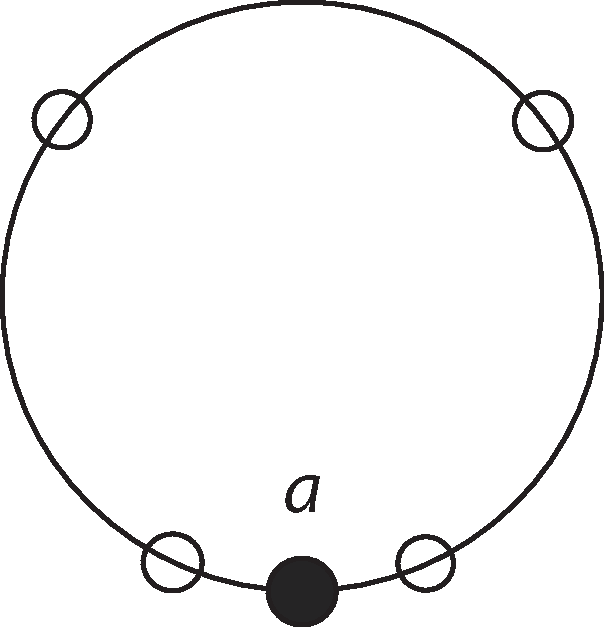
\includegraphics[width=0.44\textwidth]{images/LH035,14,02_110r-d1.pdf}
\end{minipage}
\hspace*{5mm}
\begin{minipage}[t]{0.5\textwidth}
%\hspace*{-5mm}
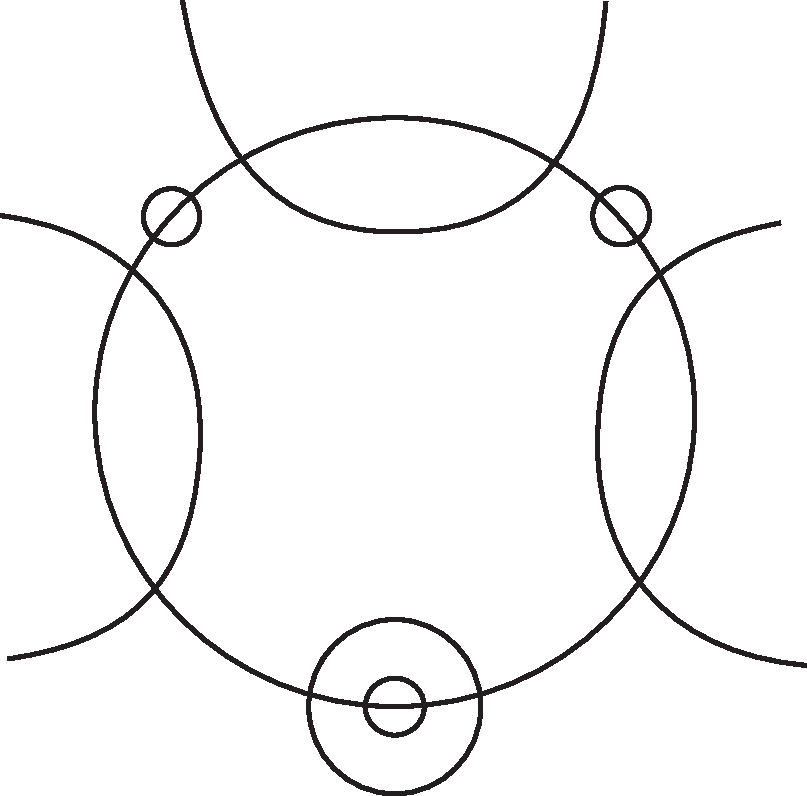
\includegraphics[width=0.56\textwidth]{images/LH035,14,02_110r-d2.pdf}
\vspace{0.8em}
\end{minipage}
\hspace*{21mm} [\textit{Fig. 1}]\hspace*{59mm} [\textit{Fig. 2}] \edtext{}{\lemma{[\textit{Fig. 1}]}\killnumber\Cfootnote{Siehe Abbildung \cite{01032}\cite{01029}a.a.O., S. 652.}}
\edtext{}{\lemma{\hspace*{1.8mm}[\textit{Fig. 2}]}\killnumber\Cfootnote{Siehe Abbildung \cite{01032}\cite{01029}a.a.O., S. 661b.}}
\pend
\newpage
\count\Afootins=1500
\count\Bfootins=1500
\count\Cfootins=1500
\pstart
[109v\textsuperscript{o}]
Tomus IV Gassendi\protect\index{Namensregister}{\textso{Gassendi} (Gassendus), Pierre 1592-1655}
est de rebus Astronomicis,
at 3\textsuperscript{tius} continet opuscula philosophica.
In iis primum
\edtext{\textit{Instit. Astron.}}{\lemma{\textit{Instit. Astron.}}\Cfootnote{P. \textsc{Gassendi}, \cite{01033}\textit{Institutio astronomica iuxta hypotheseis tam veterum quam Copernici et Tychonis Brahei}, \cite{01029}\textit{GOO} IV, S. 1-65.}}
deinde observationes coelestes titulo
\edtext{\textit{Commentariorum}}{\lemma{\textit{Commentariorum}}\Cfootnote{P. \textsc{Gassendi}, \cite{01034}\textit{Commentarii de rebus caelestibus}, \cite{01029}\textit{GOO} IV, S. 75-498.}}
\textit{de rebus coelestibus.}
Habet observationes
\edtext{de Cometa\protect\index{Sachverzeichnis}{cometa} 1618}{\lemma{de Cometa 1618}\Cfootnote{%
\cite{01034}\cite{01029}a.a.O.,
% P. \textsc{Gassendi}, \textit{Commentarii de rebus caelestibus}, anno 1618, \textit{GOO} IV,
S. 77-79.}},
eum non habuisse Parallaxim\protect\index{Sachverzeichnis}{parallaxis} sensibilem,
nisi minorem sole\protect\index{Sachverzeichnis}{Sol},
et perinde fuisse supra solem, ab anno 18 inde saepe observavit,
etiam \edtext{cometam\protect\index{Sachverzeichnis}{cometa} 1652}{\lemma{cometam 1652}\Cfootnote{%
\cite{01034}\cite{01029}a.a.O.,
% P. \textsc{Gassendi}, \textit{Commentarii de rebus caelestibus}, appendix, \textit{GOO} IV,
S. 481-498.}}.
In \edtext{Epistola Gassendi\protect\index{Namensregister}{\textso{Gassendi} (Gassendus), Pierre 1592-1655}
ad Schickardum\protect\index{Namensregister}{\textso{Schickard} (Schickardus), Wilhelm 1592-1635}
de \textit{Mercurio\protect\index{Sachverzeichnis}{Mercurius}
in sole\protect\index{Sachverzeichnis}{Sol}
viso et Venere\protect\index{Sachverzeichnis}{Venus}
invisa},}{\lemma{Epistola [...] \textit{invisa}}\Cfootnote{%
P. \textsc{Gassendi}, \cite{01035}\textit{Mercurius in sole visus et Venus invisa Parisiis anno 1631}, \cite{01029}\textit{GOO} IV, S. 499-510.}}
\edtext{cum Mercurius\protect\index{Sachverzeichnis}{Mercurius}
\edtext{esset in sole, longe minorem ordinario apparuisse,
unius diametri ejus apparentem}{\lemma{esset in sole,}\Bfootnote{\textit{(1)}\ non sui appar \textit{(2)}\ longe [...] apparentem \textit{L}}}
non esse minuto majorem etiam cum est akronychius.}{\lemma{cum Mercurius [...] akronychius}\Cfootnote{%
\cite{01035}\cite{01029}a.a.O.,
%P. \textsc{Gassendi}, \textit{Mercurius in sole visus}, epist. prior, \textit{GOO} IV,
S. 502a; 501a.}}
\edtext{Keplerus\protect\index{Namensregister}{\textso{Kepler} (Keplerus), Johannes 1571-1630}
recte praedixerat visum iri Martem\protect\index{Sachverzeichnis}{Mars}
sub sole\protect\index{Sachverzeichnis}{Sol}
at Venus\protect\index{Sachverzeichnis}{Venus} non apparuit.
Ergo de motu ejus error.}{\lemma{Keplerus [...] error}\Cfootnote{%
\cite{01035}\cite{01029}a.a.O.,
% P. \textsc{Gassendi}, \textit{Mercurius in sole visus}, epist. posterior, \textit{GOO} IV,
S. 505a-b.
Siehe J. \textsc{Kepler}, \cite{01037}\textit{Admonitio ad astronomos}, Frankfurt 1630.}}
\pend
\count\Bfootins=1500
\count\Cfootins=1500
\count\Afootins=1500
\pstart
\edtext{\textit{Novem stellae\protect\index{Sachverzeichnis}{stella}
circa Jovem\protect\index{Sachverzeichnis}{Iuppiter} visae,
Coloniae\protect\index{Ortsregister}{K\"{o}ln}
1642 et 1643} et de iis [judicia]\edtext{}{\Bfootnote{judicii \textit{\ L \"{a}ndert Hrsg.}}}
Petri Gassendi\protect\index{Namensregister}{\textso{Gassendi} (Gassendus), Pierre 1592-1655},
\textit{accessit relatio observationis
perpendiculorum\protect\index{Sachverzeichnis}{perpendiculum}
bis in die
aestus maris\protect\index{Sachverzeichnis}{aestus maris}
instar reciprocantium.}}{\lemma{\textit{Novem} [...] \textit{reciprocantium}}\Cfootnote{%
P. \textsc{Gassendi}, \cite{01036}\textit{Novem stellae circa Iovem visae%
% Coloniae exeunte anno 1642 et ineunte 1643. Et de eisdem Petri Gassendi iudicium epistola singulari contentum. Accessit relatio observationis perpendiculorum bis in die (aestus Maris instar) reciprocantium, factae a nobili Peirinsio
}, \cite{01029}\textit{GOO} IV, S. 511-522.}}
\edtext{Rheita\protect\index{Namensregister}{\textso{Schyrl} (Schyrlaeus de Rheita), Anton Maria 1597-1660}
5 novos appellabat
Urban-octavianos.}{\lemma{Rheita [...] Urban-octavianos}\Cfootnote{%
\cite{01036}\cite{01029}a.a.O.,
% P. \textsc{Gassendi},\textit{Novem stellae}, epist. A.M. De Rheita ad E. Puteanum, \textit{GOO} IV,
S. 513a.}}
\edtext{Gassendus\protect\index{Namensregister}{\textso{Gassendi} (Gassendus), Pierre 1592-1655}
conjicit fuisse fixas,\protect\index{Sachverzeichnis}{stella fixa}
in litera ad Naudaeum;\protect\index{Namensregister}{\textso{Naud\'{e}} (Naudaeus), Gabriel 1600-1653}%
}{\lemma{Gassendus [...] ad Naudaeum}\Cfootnote{%
\cite{01036}\cite{01029}a.a.O.,
% P. \textsc{Gassendi}, \textit{Novem stellae}, epist. ad G. Naudaeum, \textit{GOO} IV,
S. 517a.}}
\edtext{adjicit
\textit{postscriptum de observata gemina in singulos dies
aestus maris\protect\index{Sachverzeichnis}{aestus maris}
instar perpendiculorum\protect\index{Sachverzeichnis}{perpendiculum} reciprocatione}[,]
observata a nobili Delphinate,
Alexandro Calignono Peirinsio\protect\index{Namensregister}{\textso{Peirinsius}, Alexander Calignonus},
et per Jacobum Valesium\protect\index{Namensregister}{\textso{Valesius}, Jacobus}
Franciae thesaurarium communicata.
Vir est perspectae solertiae, industriae, eruditionis,
fidei.}{\lemma{adjicit [...] fidei}\Cfootnote{%
\cite{01036}\cite{01029}a.a.O.,
% P. \textsc{Gassendi}, \textit{Novem stellae}, epist. ad G. Naudaeum, postscriptum, \textit{GOO} IV,
S. 520b.}}
Nimirum
\edtext{ex Galilaei\protect\index{Namensregister}{\textso{Galilei} (Galilaeus, Galileus), Galileo 1564-1642}
hypothesi}{\lemma{ex Galilaei hypothesi}\Cfootnote{%
G. \textsc{Galilei}, \cite{00277}\textit{Dialogo}, Florenz 1632, giornata IV.}}
collegit
%%%%%%%%%
\edtext{\textit{si verum}}{\lemma{17-S. 7.15 \textit{si verum} [...] \textit{meridiano}}\killnumber\Cfootnote{%
P. \textsc{Gassendi}, \cite{01036}\textit{Novem stellae},
\cite{01029}\textit{GOO} IV, S. 520b-521a. Zitat mit Auslassungen.}}
\textit{sit mare bis in singulos dies fluere ac refluere\protect\index{Sachverzeichnis}{fluxus et refluxus maris}
ob geminatam quotidie in motu telluris\protect\index{Sachverzeichnis}{motus Telluris} inaequalitatem,
debere quoque pendulum,\protect\index{Sachverzeichnis}{pendulum}
et fluitando}
latum
\textit{in aere plumbum,
ubi semel observatum fuerit conquiescere,
geminata quadam in singulos dies reciprocatione, ita}
effici,
\textit{ut} bis
\textit{intra metas expatians,
bis intra horas 24 versus utramque eat ac redeat.
Itaque perpendicula\protect\index{Sachverzeichnis}{perpendiculum}
habuit brevissimum pedum 5,
longissimum 30.
meditatur unum 30 orgyarum}[,]
fili prolixitas tubo inclusa continetur.
\textit{Parato plumbo cum cuspidula inferne conspicua,
expectavit primum quousque illud conquievit penitus,
ac ipsi deinde supposuit infixam cubo cuspidulam,
quae impendenti alii directe et quam proxime responderet.
Observavit autem non constare cuspidulam plumbi super baseos cuspidulam,
sed senis horis in boream,\protect\index{Sachverzeichnis}{Borea}
senis in austrum\protect\index{Sachverzeichnis}{Auster} divergere;
\edtext{idque}{\lemma{}\Afootnote{\textit{Nach} idque: NB.}}
non sine deflexione aliqua ex Borea\protect\index{Sachverzeichnis}{Borea}
in ortum aut ex meridie in occasum.
Rem accuratius exploraturus,
cum observasset limitem excursus
in austrum\protect\index{Sachverzeichnis}{Auster}
attingi ipso meridie;
ac praeterea in media nocte,
ideo libellato primum pavimento,
et plumbo ad ipsum proxime demisso,
adnotavit hora meridiana punctum
cui cuspidula plumbi immineret,
ac deinceps}
traduxit
\textit{per ipsum, meridianam lineam.
Fixit postea in eodem puncto brevissimam cuspidulam
quam indicem dixit,
habuitque tum pro austrino\protect\index{Sachverzeichnis}{Australis, Austrinus}
limite a quo mensuraret digressionem in boream,\protect\index{Sachverzeichnis}{Borea}
tum pro centro cujus respectu,
et per ductum proxime arcum
deviationem a meridiano.}
%}{\lemma{\textit{si verum} [...] \textit{meridiano}}\Cfootnote{%
%P. \textsc{Gassendi}, \cite{01036}\textit{Novem stellae},
%\cite{01029}\textit{GOO} IV, S. 520b-521a. Zitat mit Auslassungen.}}
\edtext{\textit{Quovis die
perpendiculum\protect\index{Sachverzeichnis}{perpendiculum}
sic excurrere a Borea in austrum,
et recurrere ab austro\protect\index{Sachverzeichnis}{Auster}
in Boream\protect\index{Sachverzeichnis}{Borea}},
et meridie pervenire ad limitem austrinum,\protect\index{Sachverzeichnis}{Australis, Austrinus}
\edtext{ut et}{\lemma{ut et}\Bfootnote{\textit{erg. L}}}
media \edtext{nocte; at vero \textit{ad Boream\protect\index{Sachverzeichnis}{Borea}}%
}{\lemma{nocte;}\Bfootnote{\textit{(1)} ad borealem\ \textit{(2)} at vero \textit{ad Boream}\ \textit{L}}}
\textit{hora sexta tam matutina quam vespertina,
ac sit in medio itineris tum excurrendo hora nona,
tum recurrendo tertia circum meridiem mediamque noctem.
Esse tam excursum quam recursum in medio praesertim velocem}[,]
\textit{in limitibus potissimum lentum,
nam ad austrinum\protect\index{Sachverzeichnis}{Australis, Austrinus}
v.g. limitem dum attenditur}[,]
\textit{ipsam plumbi cuspidulam haerere super indicem,
neque evariari sensibiliter per unam alteramve horam.
Tertio Austrinum\protect\index{Sachverzeichnis}{Australis, Austrinus}
limitem esse constantiorem quam Boream,\protect\index{Sachverzeichnis}{Borea}
vix enim unquam ab illo quicquam versus occidentem procurri,
at ab isto saepe versus orientem
plurimum},
deque illa evagatione illi nondum posse aliquid definiri[;]
observatio per plusquam mensem constanter repetita.}{\lemma{\textit{Quovis} [...] repetita}\Cfootnote{%
\cite{01036}\cite{01029}a.a.O., S. 521a. Zitat mit Auslassungen.}}
Hinc demonstrare conatur,
fieri accessum et recessum maris\protect\index{Sachverzeichnis}{accessus et recessus maris} non ab ortu in
\edtext{occasum et contra}{\lemma{occasum}\Bfootnote{\textit{(1)}\ sed \textit{(2)}\ et contra \textit{L}}}
cum Galilaeo\protect\index{Namensregister}{\textso{Galilei} (Galilaeus, Galileus), Galileo 1564-1642}
sed a borea\protect\index{Sachverzeichnis}{Borea}
in austrum\protect\index{Sachverzeichnis}{Auster}
vel contra.
Rem variis experimentis declarat,
\edtext{sed illud}{\lemma{27-S. 8.8 \hspace{1.3mm}sed illud [...] \textit{polum}}\killnumber\Cfootnote{%
\cite{01036}\cite{01029}a.a.O., S. 521a-b. Zitat mit Auslassungen.}} appositum maxime
\textit{de figuli rota\protect\index{Sachverzeichnis}{rota figuli},}
\pend
\newpage
\pstart \noindent \textit{deque pelvi aut situla super eam ita constituta
ut medium vel centrum superficiei aquae intra vas contentae}
[111~r\textsuperscript{o}]
\textit{ipsi rotae centro}
exacte
\textit{respondeat.
Nempe si rota post lentam motionem torqueatur concitatius,
aqua ipso medio in quendam velut umbilicum excavato dilabitur,
et versus oram exturbatur,
et si rota postea agatur remissius
aqua ex ora relabitur ac se in medium recipit.
Ita in globo}
terrae\protect\index{Sachverzeichnis}{globus}
\textit{si circumvolvi admittatur}[,]
si \textit{habeat aequator\protect\index{Sachverzeichnis}{aequator} rationem orae,
et polus\protect\index{Sachverzeichnis}{polus}
uterque medii seu umbilici,
necesse est aquam increscente motus
velocitate\protect\index{Sachverzeichnis}{velocitas}
diffluere a polo versus aequatorem
et decrescente refluere ex aequatore\protect\index{Sachverzeichnis}{aequator}
versus polum.\protect\index{Sachverzeichnis}{polus}}%
%}{\lemma{sed illud [...] \textit{polum}}\Cfootnote{%
%\cite{01036}\cite{01029}a.a.O., S. 521a-b. Zitat mit Auslassungen.}}
Notabile illud quoque
quod \edtext{observationes ejus testantur excurrere et recurrere
perpendiculum\protect\index{Sachverzeichnis}{perpendiculum}
quasi ex Caecia\protect\index{Sachverzeichnis}{Caecia}
in Africum\protect\index{Sachverzeichnis}{Africus} et contra,
non intra Boream\protect\index{Sachverzeichnis}{Borea}
et Austrum\protect\index{Sachverzeichnis}{Auster}
praecise.
Ita fieri scilicet fluxum et refluxum maris\protect\index{Sachverzeichnis}{fluxus et refluxus maris}
quoque cum aqua non directe ex medio
\textit{in oram, sed oblique
quasi quibusdam spiris factis aufugiat et
refugiat.}
Cumque parallelus viri sit inter
polum\protect\index{Sachverzeichnis}{polus}
et aequatorem\protect\index{Sachverzeichnis}{aequator}
medius,
\textit{perpendiculorum\protect\index{Sachverzeichnis}{perpendiculum}
excursus et recursus obliquitate media fient}[,]
prope polos\protect\index{Sachverzeichnis}{polus} magis accedent
\edtext{ad austroborealem.}{\lemma{ad}\Bfootnote{\textit{(1)}\ boream \textit{(2)}\ meridianam inter \textit{(3)}\ austroborealem \textit{L}}}}{\lemma{observationes [...] austroborealem}\Cfootnote{%
\cite{01036}\cite{01029}a.a.O., S. 521b, mit Auslassungen.}}
\edtext{Sed an non deberet etiam in pleniluniis et noviluniis major esse motus
\edtext{perpendiculi\protect\index{Sachverzeichnis}{perpendiculum}}{\lemma{perpendiculi}\Bfootnote{\textit{erg. L}}}
ut \edtext{aestus.\protect\index{Sachverzeichnis}{aestus maris}
At}{\lemma{aestus.}\Bfootnote{\textit{(1)}\ An \textit{(2)}\ At \textit{L}}}
cum semel solum dietim velocitas\protect\index{Sachverzeichnis}{velocitas}
motus telluris\protect\index{Sachverzeichnis}{motus Telluris} increscat,
ad noctem mediam,
cur perpendiculum\protect\index{Sachverzeichnis}{perpendiculum}
bis recurrit?
An quod excursus uno vi verticitatis terrae absoluto alius
\edtext{peragatur solo ponderis\protect\index{Sachverzeichnis}{pondus}%
}{\lemma{peragatur}\Bfootnote{\textit{(1)}\ vi \textit{(2)}\ solo ponderis \textit{L}}}
prolapsu, et idem fiat in motu maris\protect\index{Sachverzeichnis}{motus maris},
ita, ut altera itio, sit tantum repetitio prioris,
at tertia rursus ex nova impressione.
An dicendum perpendiculum\protect\index{Sachverzeichnis}{perpendiculum} ita nutare,
quod terra vacillet[,]
eam autem vacillare a centro gravitatis\protect\index{Sachverzeichnis}{centrum gravitatis}
aquarum motu variato.
Qui deinde a luna[?]\protect\index{Sachverzeichnis}{Luna}
\edtext{At luna quod}{\lemma{At}\Bfootnote{\textit{(1)}\ si \textit{(2)}\ luna quod \textit{L}}} aerem premit,
cum non sit membranae inclusus, et si esset,
cur non nos aeque ac mare?}{\lemma{Sed an [...] mare?}\Cfootnote{%
\cite{01036}\cite{01029}a.a.O., S. 521b-522a.}}
(Responderi potest \edtext{experimentis
Pascalii\protect\index{Namensregister}{\textso{Pascal} (Pascalius), Blaise 1623-1662}
de pressione\protect\index{Sachverzeichnis}{pressio}%
}{\lemma{experimentis [...] de pressione}\Cfootnote{%
B. \textsc{Pascal}, \cite{00081}\textit{Trait{\'e} de l'{\'e}quilibre des liqueurs}, Paris 1663.
Siehe dazu Leibniz' Exzerpte in \cite{001038}\textit{LSB} VIII, 1 N. 38.}})
Gellibrandi\protect\index{Namensregister}{\textso{Gellibrand} (Gellibrandus), Henry 1597-1636}
\edtext{opusculum}{\lemma{opusculum}\Cfootnote{%
H. \textsc{Gellibrand}, \cite{00288}\textit{A discourse mathematical on the variation of the magnetical needle}, London 1635.}}
admonuit variationem magneticam\protect\index{Sachverzeichnis}{variatio magnetica} mutari.
\pend
\count\Bfootins=1500
\count\Cfootins=1500
\count\Afootins=1500
%%%%